% Created: 2019-12-10
% Plot participant data
% http://github.com/zhaobn/magic_stones

\documentclass{article}
\title{[Magic Stones] Report for Complete Experiment 1}
\author{Bonan Zhao (b.zhao@ed.ac.uk)}

% Text formats: margin, font, spacing
\usepackage[margin=0.8in]{geometry}
\usepackage{charter}
\renewcommand{\baselinestretch}{1.3}

% Graphics
\usepackage{graphicx}
\usepackage{subcaption}
\graphicspath{{../figs/}}

\usepackage{amsmath}

\begin{document}
\maketitle

% Raw participant data
\section{Participant data}

\begin{figure}[h!]
	\centering
  \begin{subfigure}[t]{0.32\textwidth}
  	\centering
  	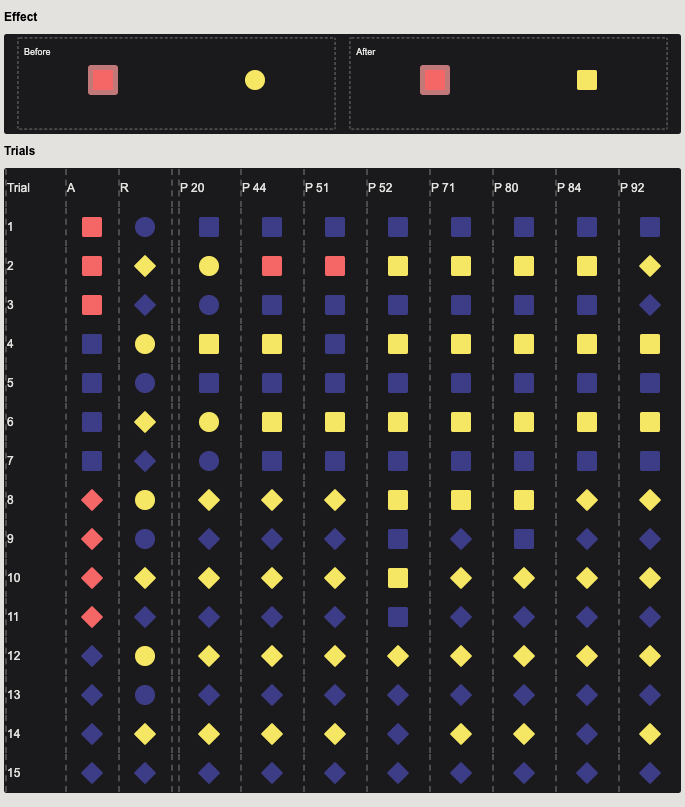
\includegraphics[width=\linewidth]{learn01} 
  	\caption{To the same shape} \label{fig:learn01}
  \end{subfigure}
  \hfill
  \begin{subfigure}[t]{0.32\textwidth}
  	\centering
  	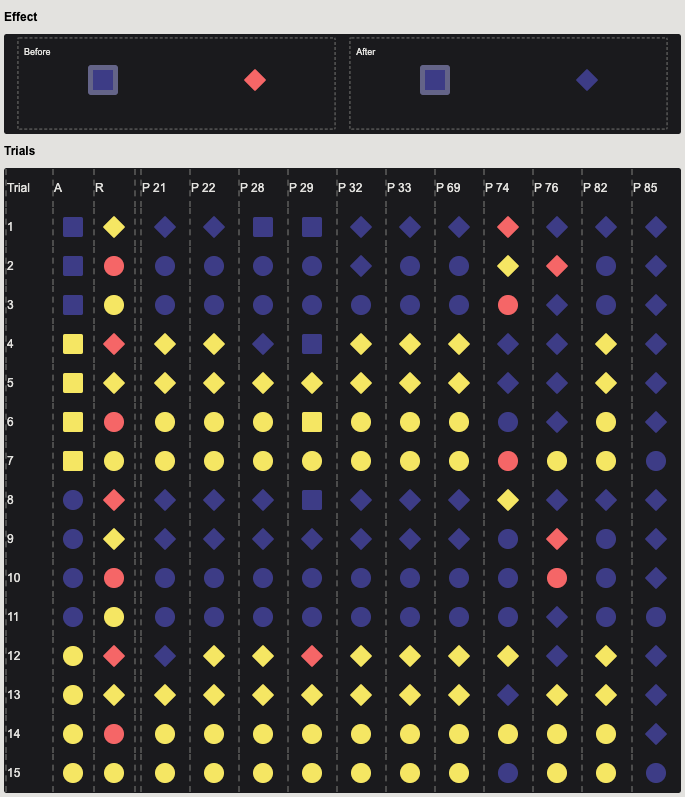
\includegraphics[width=\linewidth]{learn03} 
  	\caption{To the same color} \label{fig:learn03}
  \end{subfigure}
  \hfill
  \begin{subfigure}[t]{0.32\textwidth}
  	\centering
  	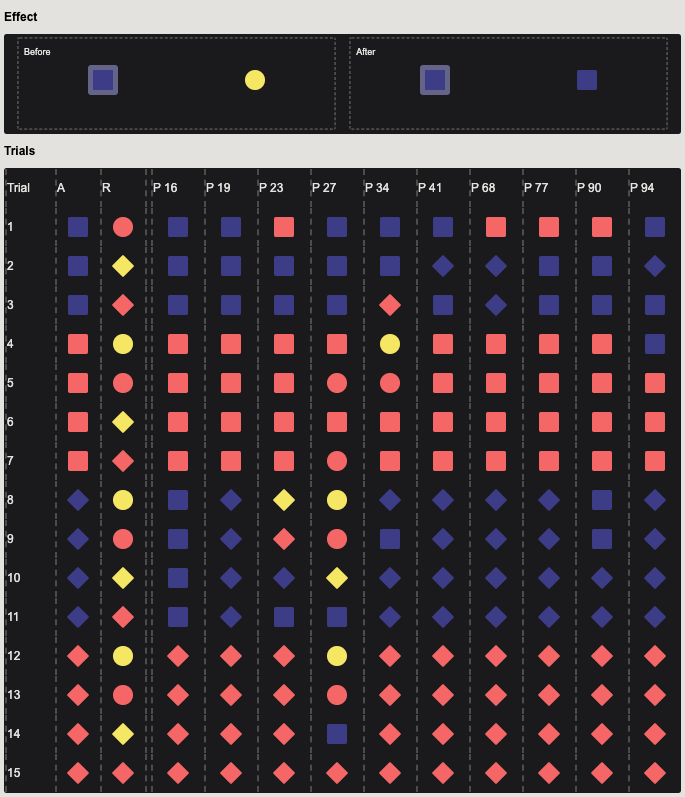
\includegraphics[width=\linewidth]{learn06} 
  	\caption{To the same object} \label{fig:learn06}
  \end{subfigure}

  \vspace{1em}
  \begin{subfigure}[t]{0.32\textwidth}
  	\centering
  	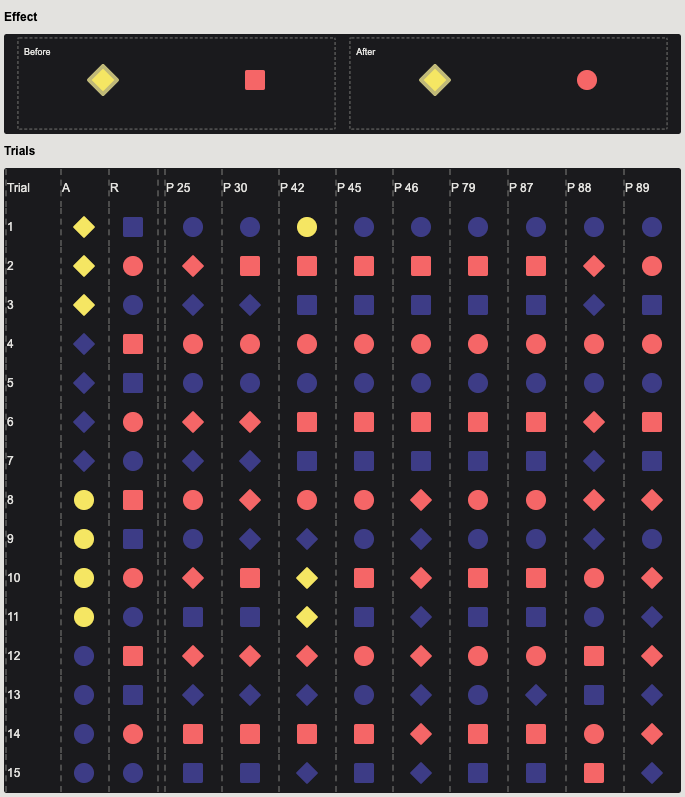
\includegraphics[width=\linewidth]{learn02} 
  	\caption{To a different shape} \label{fig:learn02}
  \end{subfigure}
  \hfill
  \begin{subfigure}[t]{0.32\textwidth}
  	\centering
  	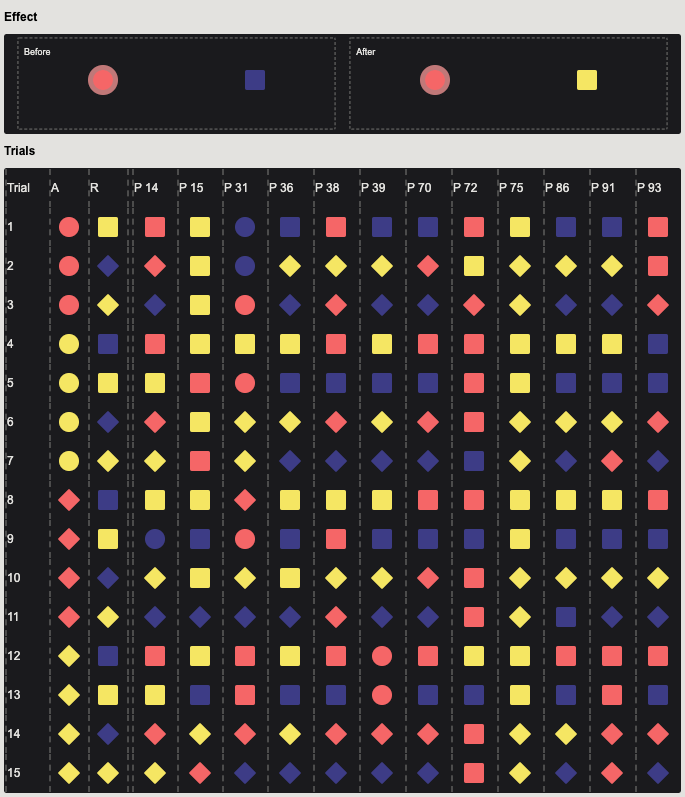
\includegraphics[width=\linewidth]{learn04} 
  	\caption{To a different color} \label{fig:learn04}
  \end{subfigure}
  \hfill
  \begin{subfigure}[t]{0.32\textwidth}
  	\centering
  	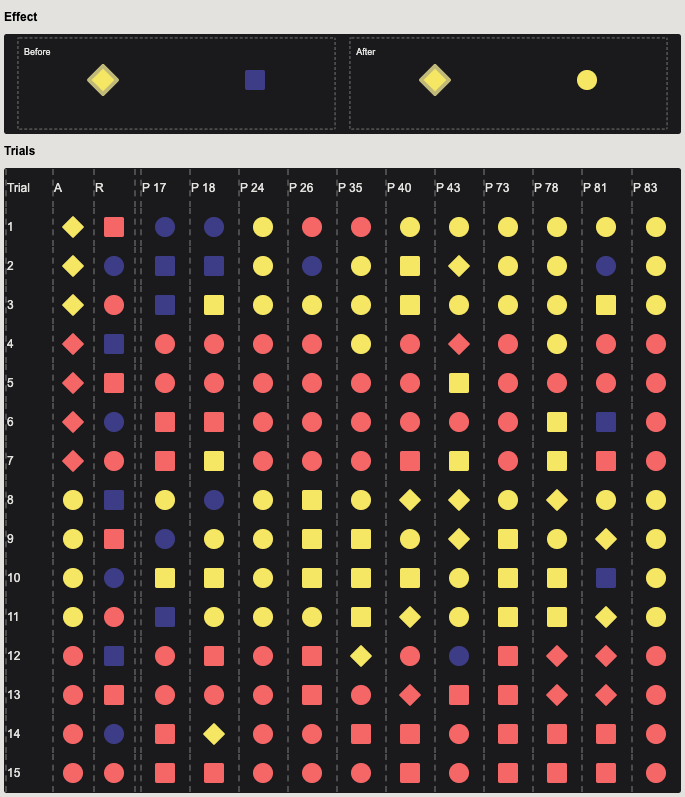
\includegraphics[width=\linewidth]{learn05} 
  	\caption{To a different object} \label{fig:learn05}
  \end{subfigure}
  \caption{Each figure is for one learning condition. 
  Each learning condition has 15 trials (15 rows).}
\end{figure}




\end{document}